\documentclass[bachelor, och, coursework]{SCWorks}
% параметр - тип обучения - одно из значений:
%    spec     - специальность
%    bachelor - бакалавриат (по умолчанию)
%    master   - магистратура
% параметр - форма обучения - одно из значений:
%    och   - очное (по умолчанию)
%    zaoch - заочное
% параметр - тип работы - одно из значений:
%    referat    - реферат
%    coursework - курсовая работа (по умолчанию)
%    diploma    - дипломная работа
%    pract      - отчет по практике
% параметр - включение шрифта
%    times    - включение шрифта Times New Roman (если установлен)
%               по умолчанию выключен
\usepackage{subfigure}
\usepackage{tikz,pgfplots}
\pgfplotsset{compat=1.5}
\usepackage{float}

%\usepackage{titlesec}
\setcounter{secnumdepth}{4}
%\titleformat{\paragraph}
%{\normalfont\normalsize}{\theparagraph}{1em}{}
%\titlespacing*{\paragraph}
%{35.5pt}{3.25ex plus 1ex minus .2ex}{1.5ex plus .2ex}

\titleformat{\paragraph}[block]
{\hspace{1.25cm}\normalfont}
{\theparagraph}{1ex}{}
\titlespacing{\paragraph}
{0cm}{2ex plus 1ex minus .2ex}{.4ex plus.2ex}

% --------------------------------------------------------------------------%


\usepackage[T2A]{fontenc}
\usepackage[utf8]{inputenc}
\usepackage{graphicx}
\graphicspath{ {./images/} }
\usepackage{tempora}

\usepackage[sort,compress]{cite}
\usepackage{amsmath}
\usepackage{amssymb}
\usepackage{amsthm}
\usepackage{fancyvrb}
\usepackage{listings}
\usepackage{listingsutf8}
\usepackage{longtable}
\usepackage{array}
\usepackage[english,russian]{babel}

% \usepackage[colorlinks=true]{hyperref}
\usepackage{url}

\usepackage{underscore}
\usepackage{setspace}
\usepackage{indentfirst} 
\usepackage{mathtools}
\usepackage{amsfonts}
\usepackage{enumitem}
\usepackage{tikz}
\usepackage{minted}

\newcommand{\eqdef}{\stackrel {\rm def}{=}}
\newcommand{\specialcell}[2][c]{%
\begin{tabular}[#1]{@{}c@{}}#2\end{tabular}}

\renewcommand\theFancyVerbLine{\small\arabic{FancyVerbLine}}

\newtheorem{lem}{Лемма}

\begin{document}

% Кафедра (в родительном падеже)
\chair{теоретических основ компьютерной безопасности и криптографии}

% Тема работы
\title{Генерация текстового описания к изображению с помощью нейронной сети}

% Курс
\course{3}

% Группа
\group{331}

% Факультет (в родительном падеже) (по умолчанию "факультета КНиИТ")
\department{факультета КНиИТ}

% Специальность/направление код - наименование
%\napravlenie{09.03.04 "--- Программная инженерия}
%\napravlenie{010500 "--- Математическое обеспечение и администрирование информационных систем}
%\napravlenie{230100 "--- Информатика и вычислительная техника}
%\napravlenie{231000 "--- Программная инженерия}
\napravlenie{100501 "--- Компьютерная безопасность}

% Для студентки. Для работы студента следующая команда не нужна.
% \studenttitle{Студентки}

% Фамилия, имя, отчество в родительном падеже
\author{Улитина Ивана Владимировича}

% Заведующий кафедрой
\chtitle{} % степень, звание
\chname{Абросимов М. Б.}

%Научный руководитель (для реферата преподаватель проверяющий работу)
\satitle{доцент} %должность, степень, звание
\saname{Слеповичев И. И.}

% Руководитель практики от организации (только для практики,
% для остальных типов работ не используется)
% \patitle{к.ф.-м.н.}
% \paname{С.~В.~Миронов}

% Семестр (только для практики, для остальных
% типов работ не используется)
%\term{8}

% Наименование практики (только для практики, для остальных
% типов работ не используется)
%\practtype{преддипломная}

% Продолжительность практики (количество недель) (только для практики,
% для остальных типов работ не используется)
%\duration{4}

% Даты начала и окончания практики (только для практики, для остальных
% типов работ не используется)
%\practStart{30.04.2019}
%\practFinish{27.05.2019}

% Год выполнения отчета
\date{2022}

\maketitle

% Включение нумерации рисунков, формул и таблиц по разделам
% (по умолчанию - нумерация сквозная)
% (допускается оба вида нумерации)
% \secNumbering

%-------------------------------------------------------------------------------------------

\tableofcontents

\intro

    Последнее десятилетие имплементации алгоритмов искусственного интеллекта раз за разом поражали людей своими
    способностями решать задачи, считавшиеся до этого выполнимыми исключительно человеком. И с каждым годом темп
    развития этой сферы информационных технологий многократно увеличивался, всё сильнее поражая людей обширностью
    потенциала и возможностей использования глубокого обучения в повседневной жизни, которая постепенно преображалась в
    силу движения прогресса. В современном мире так много приложений нейросетевых алгоритмов в самых различных отраслях
    человеческой жизнедеятельности, что всё чаще человек использует ИИ, иногда даже не подозревая об этом. От нахождения
    кратчайшего пути из дома до аэропорта и прогнозирования погоды по параметрам воздуха и вплоть до удовлетворения
    банковских услуг пользователя с помощью автоответчика "--- всё это напрямую говорит об удивительном множестве
    возможностей использования искусственного интеллекта, которое постоянно расширяется.
    
    Среди разделов глубокого обучения, использование которых ввергает людей в восхищение перед возможностями ИИ, следует
    выделить \textbf{NLP} и \textbf{Computer Vision}. В данной работе пойдёт речь именно о такой совокупности
    нейросетей, которая будет осуществлять обработку изображения таким образом, чтобы ко входному для алгоритма рисунку
    генерировалось текстовое описание. Чаще всего, в англоязычных ресурсах данная задача называется \textbf{Image
    Captioning}, и реализации её решения являются прикладной технологией для самых различных нужд.

    % Вероятно, будет полезно в тех случаях, когда чаще всего используется текст, и с его помощью вы можете
    % вывести/генерировать текст из изображений. Например, использовать информацию непосредственно из любого конкретного
    % изображения в текстовом формате автоматически. В настоящее время существует множество приложений НЛП, которые
    % извлекают информацию/резюме из заданных текстовых данных, эссе и т. д. Те же преимущества могут быть получены
    % людьми, которые выиграют от автоматизированного анализа изображений. Слегка (не очень) долгосрочным вариантом
    % использования, безусловно, было бы объяснение того, что происходит в видео, кадр за кадром. Послужит огромным
    % подспорьем для слабовидящих людей. В этом пространстве можно разработать множество приложений. Социальные сети.
    % Такие платформы, как Facebook, могут делать выводы непосредственно из изображения, где вы находитесь (пляж, кафе и
    % т. д.), что вы носите (цвет) и, что более важно, что вы делаете (в каком-то смысле). Посмотрите пример, чтобы
    % лучше понять его.

\defabbr

    Перед анализом теоретической составляющей глубокого обучения и архитектур нейронных сетей, которые осуществляют
    генерацию текстового описания к входному для алгоритма изображению, стоит ввести ряд терминов и определений,
    являющихся основой для понимания работы алгоритма генерации.

    \textit{Искусственный интеллект} (англ. Artificial Intelligence) "--- технология создания алгоритмов, лежащих в
    основе проектирования интеллектуальных машин и программ, способных имитировать деятельность человека.

    \textit{Нейронная сеть (нейросеть)} (англ. Neural Network) "--- математическая модель, чаще всего имеющая
    программную интерпретацию, сутью которой является реализация деятельности, похожей на деятельность биологических
    нейронных сетей. Нейронная сеть используется при создании какого-либо из алгоритмов искусственного интеллекта и
    состоит из совокупности нейронов, соединенных между собой связями. 

    \textit{Признак} (англ. Feature) "--- каждый отдельный элемент информации, включаемый в представление о каком-либо
    анализируемом объекте.

    \textit{Машинное обучение} (англ. Machine Learning) "--- область науки об искусственном интеллекте, которая изучает
    способы создания алгоритмов, которые могут обучаться (развиваться).

    \textit{Глубокое обучение} (англ. Deep Learning) "--- частный случай машинного обучения, который представляет из
    себя методы машинного обучения, основанные на обучении представлений. Осуществляет получение представлений путем их
    выражения через более простые представления, а формирование последних, в свою очередь, реализуется через ещё более
    простые представления, и так далее.

    \textit{Компьютерное зрение} (англ. Computer Vision) "--- область науки об искусственном интеллекте, использующая
    методы машинного и глубокого обучения для решения задач распознавания, классификации, мониторинга с помощью
    получения необходимой информации из изображения.

    \textit{Обработка естественного языка} (англ. Natural Language Processing, NLP) "--- направление развития ИИ и
    математической лингвистики, которое изучает проблемы синтеза и компьютерного анализа текстов на естественных языках.
    Говоря об искусственном интеллекте, под анализом подразумевается понимание языка, а под синтезом "--- генерация
    грамотного с точки зрения языковых норм текста.

    \textit{Текстовое описание к изображению} (англ. Image Captioning) "--- это задача описания содержания изображения
    словами естественного языка. Принцип решения лежит на пересечении таких разделов глубокого обучения как
    компьютерного зрения и обработки естественного языка. В большинстве систем генерации текстовых описаний к
    изображениям используется структура кодировщик-декодер, в которой входное изображение кодируется в промежуточное
    представление информации о содержимом изображения, а затем декодируется в описательную текстовую последовательность.

\section{Теоретическая часть}

    \subsection{Сверточная нейронная сеть}

        % Принцип работы
        Искусственные нейронные сети или ИНС (англ. Artificial Neural Network или ANN) "--- это системы вычислительной
        обработки, принцип работы которых в значительной степени основан на том, как работают биологические нервные
        системы (в частности, человеческий мозг). ИНС в основном состоят из большого количества взаимосвязанных
        вычислительных узлов (называемых нейронами), работа которых определяется соединениями со слоями, содержащими
        другие нейроны. В итоге совокупность вычислений, производимых этими нейронами, осуществляет процесс обучения,
        который заключается в минимизации ошибки окончательного вывода нейросети (т.е. результата её работы).
        
        Сверточные нейронные сети (англ. Convolutional Neural Network, CNN) аналогичны традиционным ANN в том, что они
        состоят из нейронов, которые самооптимизируются посредством обучения. Принцип, при котором каждый нейрон
        получает входные данные и выполняет операцию (например, скалярное произведение, за которым следует применение
        нелинейной функции) "--- это основа бесчисленных вариантов реализаций ИНС. Организовывая процесс преобразования
        входных необработанных векторов изображений в некоторый окончательный результат (будь то обработка изображения,
        классификация изображения или генерация текстовой подписи), вся нейросеть по-прежнему будет представлять собой
        функции преобразования весов-коэффициентов. Последний слой будет содержать функцию потерь, определяемую классом
        решаемой задачи, и все обычные принципы организации архитектуры модели, разработанные для традиционных ИНС,
        также могут быть применимы и в работе со сверточными нейросетями. 

        Принципиальное отличие обычной нейронной сети от сверточной является наличие в последней специального
        ''сверточного'' слоя, который применяет к входным весам математическую операцию свертки. Термин свертка
        относится к математической комбинации двух функций для получения третьей функции. В случае CNN свертка
        выполняется для входных данных с использованием фильтра или ядра (эти термины взаимозаменяемы), чтобы затем
        создать карту признаков (англ. feature map). Выполнение свертки осуществляется перемещением фильтра по минорам
        входной матрицы. Для каждого минора определенного размера выполняется матричное умножение с соответствующим ему
        фильтром и суммируется результат на карте признаков. 

        \begin{figure}[H]
            \centering
            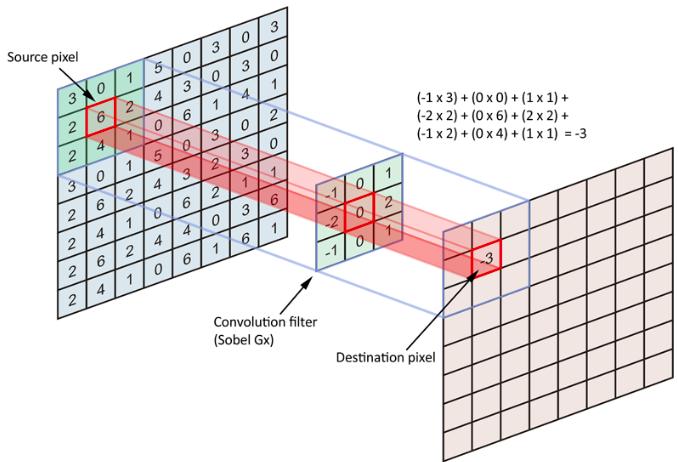
\includegraphics[width=0.8\textwidth]{pics/convolute.png}
            \caption{Операция свёртки}
        \end{figure}

        Операции свертки выполняются на входной матрице, где каждая операция использует определенный фильтр. Результатом
        итераций математической процедуры являются различные карты признаков. В качестве шага, завершающего операцию,
        берутся все эти карты признаков и объединяются вместе в качестве конечного результата сверточного слоя.

        % Область применения
        Сверточная нейронная сеть "--- это алгоритм глубокого обучения, который применяется для обработки данных с
        сеточной топологией. Один из примеров такого вида данных "--- временные ряды, которые представимы в виде
        одномерной сетки примеров, выбираемых через регулярные промежутки времени (англ. timestamp). Вторым, более
        актуальным для этой работы примером, являются изображения, которые можно интерпретировать как двумерную сетку
        пикселей.

        Популярность использования такого вида нейросетей при работе с изображениями обусловлена их отличительными
        положительными чертами. Сверточные нейронные сети обеспечивают частичную устойчивость к изменениям масштаба,
        смещениям, поворотам, смене ракурса и прочим искажениям картинки. Сверточные нейронные сети объединяют три
        архитектурных идеи, для обеспечения инвариантности к масштабируемости, вращению и другим пространственным
        деформациям:

        \begin{enumerate}
            \item локальные рецепторные поля (обеспечивают локальную двумерную связность нейронов);
            \item общие синаптические коэффициенты (обеспечивают детектирование некоторых черт в любом месте изображения
            и уменьшают общее число весовых коэффициентов);
            \item иерархическая организация с пространственными подвыборками.
        \end{enumerate}

    \subsection{Рекуррентная нейронная сеть и LSTM}

        % Принцип работы
        Рекуррентная нейронная сеть или РНС (англ. Recurrent Neural Network, RNN) "--- это тип искусственной нейронной
        сети, которая обрабатывает последовательности данных и временные ряды. Подобно нейронным сетям с прямой связью
        (англ. Feedforward Neural Network, FNN) и CNN, рекуррентные нейронные сети используют обучающие данные для
        изменения своих весов. Основным отличием от других видов сетей является ''память'', суть которой в том, что в
        процессе обработки входной информации особым текущим слоем в RNN, используются входные параметры к некоторым
        предыдущим слоям сети (таким образом влияя на результат работы текущего слоя сети). В то время как традиционные
        глубокие нейронные сети предполагают, что входные и выходные данные слоев независимы друг от друга, выходы
        рекуррентных нейронных сетей зависят от предшествующих элементов внутри последовательности этих слоев. Хотя
        будущие преобразования также могут быть полезны для определения результата данной последовательности,
        однонаправленные рекуррентные нейронные сети не могут учитывать эти преобразования в своих прогнозах.

        \begin{figure}[H]
            \centering
            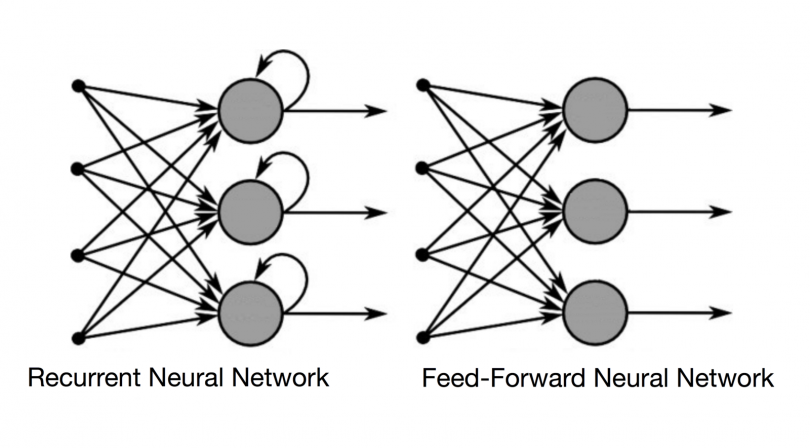
\includegraphics[width=0.8\textwidth]{pics/rnn-vs-fnn.png}
            \caption{Абстрактное сравнение архитектур FNN и RNN}
        \end{figure}

        Однако при использовании первых архитектур RNN возникала проблема потери способности связывать информацию в силу
        уменьшения влияния аргументов слоев сети на текущий обрабатываемый слой по мере увеличения ''расстояния'' между
        слоем, для которого были изначально предназначены аргументы, и текущим слоем. Уменьшение влияния выражается
        через проблему исчезающего градиента (англ. Vanishing gradient problem), которая возникает в процессе обучения
        ANN с помощью методов, основанных на градиентном спуске (англ. Gradient Descent) и методе обратного
        распространения ошибки (англ. Backpropagation). В этих способах обучения, на протяжении всей итерации обучения
        или эпохи, каждый из весов нейросети обновляется пропорционально частной производной функции ошибки от текущего
        веса. Время от времени значение градиента может становиться бесконечно малым, что препятствует обновлению
        значения веса. На практике, в силу отсутствия возможности сохранения качества передачи параметров между слоями,
        была представлена реализация модификации рекуррентной нейросети, которая способна к обучению долговременным
        зависимостям. Название такого подкласса RNN "--- сеть с долгой краткосрочной памятью (англ. Long Short-Term
        Memory, LSTM).

        Решение с помощью LSTM использует карусель с постоянными ошибками (англ. Constant Error Carousel, CEC), которые
        обеспечивают постоянный поток ошибок (необходимый для хранения значений ошибки для дальнейшего обучения модели)
        в специальных ячейках. Доступ к ячейкам (и их применение) осуществляется мультипликативными блоками ворот (англ.
        gate units), которые учатся своевременно предоставлять этот доступ. CEC являются центральной функцией LSTM, где
        осуществляется хранение краткосрочной памяти в течении длительных периодов времени. В ходе выполнения обработки
        соединений между другими блоками сети LSTM может также возникнуть конфликт обновления веса. Входные соединения
        некоторого нейрона $u$ могут конфликтовать в процессе обновления веса по причине того, что один и тот же вес
        может как использоваться для хранения некоторого входного значения, так и не использоваться. Для взвешенных
        выходов соединений, идущих от нейрона $u$, одинаковые веса могут вернуть содержимое $u$ и сделать поток вывода
        ошибки в другие нейроны сети некорректным. Эту проблему решает расширение CEC входными и выходными блоками
        ворот, которые соединены с входным слоем сети и с другими ячейками памяти, что ведет к формированию особого
        блока LSTM, называемого блоком памяти (англ. Memory Block).

        \begin{figure}[H]
            \centering
            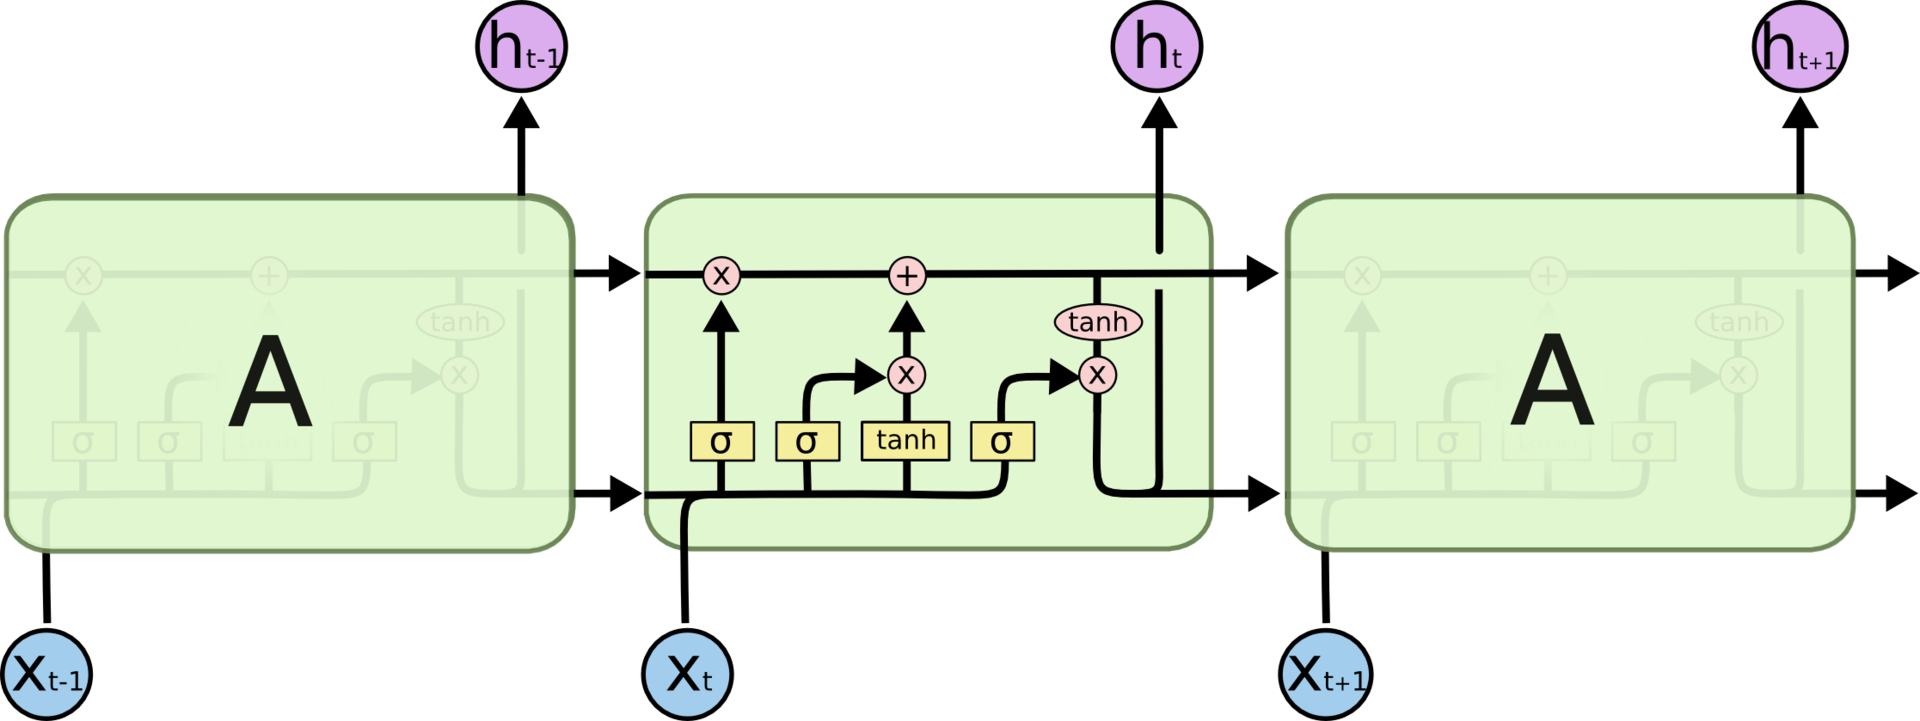
\includegraphics[width=0.8\textwidth]{pics/lstm.png}
            \caption{Схема содержимого модуля LSTM-сети}
        \end{figure}

        % Область применения
        РНС "--- это такой тип архитектуры нейронной сети, который преимущественно используется для нахождения
        закономерностей и шаблонов (англ. pattern) в последовательностях данных. Такими данными могут быть рукописи,
        представления геномов, текст или числовые временные ряды, часто используемые в рамках корпоративных задач
        машинного обучения (например, даны показатели курса некоторой акции или валюты, и требуется предсказать значение
        стоимости акции в следующий момент времени, или представлены значения сенсоров в течении некоторого временного
        промежутка и необходимо осуществить классификацию поведения этого сенсора). В общем смысле, RNN применяются в
        моделировании языка (англ. Language Modelling) и генерация текста, распознавании речи, генерации описания к
        изображениям (не только текстового, но и по возможным другим параметрам) или маркировке видео (англ. Video
        Tagging).
        
        В свою очередь, LSTM-сети (как подкласс сетей RNN) могут применяться в тех же сферах, что и обычные рекуррентные
        сети. В 2012 году модификация LSTM была применена для обнаружения ключевых слов и распознавания различных видов
        содержимого рукописных документов (такие как текст, формула, диаграмма и рисунок). Примерно в тот же период
        времени с помощью сетей с долгой краткосрочной памятью осуществлялась классификация изображений высокого
        разрешения из базы данных ImageNet, результаты которой были значительно лучше предыдущих (без использования
        LSTM). В 2015 году разновидность этого класса нейросети с использованием фреймворка Sequence-to-Sequence была
        успешно обучена для создания предложений на простом английском языке, описывающих изображения. Также в 2015 году
        LSTM была объединена с глубоким иерархическим экстрактором визуальных признаков и применена к решению задач
        интерпретации и классификации изображений, таких как определение некоторого активного действия на картинке и
        генерация описания изображения/видео.

    \subsection{Метрики оценки качества обучения}
    \subsection{Функции потерь и функции активации}
    \subsection{Задачи, решаемые генерацией текстового описания к изображению с помощью нейронной сети}

\section{Практическая часть}

    \subsection{Описание инструментов и библиотек программной реализации}

    \subsection{Описание набора данных для обучения и теста}

    \subsection{Программная реализация алгоритма}

    \subsection{Приведение характеристик обучения и гиперпараметров}

    \subsection{Результаты обучения}

\conclusion

    Здесь будет заключение

\begin{thebibliography}{99}
    \bibitem{neur} Короткий С., ''Нейронные сети: Основные положения'', [Электронный ресурс] : [статья] / URL: http://www.shestopaloff.ca/kyriako/Russian/Artificial_Intelligence/Some_publications/Korotky_Neuron_network_Lectures.pdf  (дата обращения 27.04.2021) Загл. с экрана. Яз. рус.
    % \bibitem{Gud} Гудфеллоу Я., Бенджио И., Курвилль А., ''Глубокое обучение'', г. Москва, Издательство ДМК, 2018 г., Яз. рус.
    % \bibitem{Neuron} Baestaens D. E., Van Den Bergh W. M., Wood D., ''Neural Network Solution for Trading in Financial Markets'', Pitman publishing, 1994 г., Яз. англ.
    % \bibitem{Network} Исаков С., ''Как работает сверточная нейронная сеть: архитектура, примеры, особенности'', [Электронный ресурс] : [статья] / URL: https://neurohive.io/ru/osnovy-data-science/glubokaya-svertochnaja-nejronnaja-set/ (дата обращения 27.04.2021) Загл. с экрана. Яз. рус.
    % \bibitem{Svertka} Дорогой Я., ''Архитектура обобщенных сверточных нейронных сетей'', [Электронный ресурс] : [статья] / URL: http://www.it-visnyk.kpi.ua/wp-content/uploads/2012/08/54_36.pdf (дата обращения 27.04.2021) Загл. с экрана. Яз. рус.
    % \bibitem{mathapp} Стариков А., ''Нейронные сети — математический аппарат'', [Электронный ресурс] : [сайт] / URL: https://basegroup.ru/community/articles/math (дата обращения 27.04.2021) Загл. с экрана. Яз. рус.
    % \bibitem{Gud2} Sutskever I., Martens J., Dahl G., and Hinton G., ''On the importance of initialization and momentum in deep learning.'', ICML, 2013 г., Яз. англ.

    % CNN
    % https://arxiv.org/abs/1511.08458
    % https://www.freecodecamp.org/news/an-intuitive-guide-to-convolutional-neural-networks-260c2de0a050/

    % RNN
    % https://arxiv.org/pdf/1912.05911.pdf
    % https://www.ibm.com/cloud/learn/recurrent-neural-networks
    
    % LSTM
    % https://arxiv.org/pdf/1909.09586.pdf
    % https://habr.com/ru/company/wunderfund/blog/331310/

\end{thebibliography}

\appendix

    \section{Код getloader.py}
    \inputminted[fontsize=\footnotesize]{python}{model-ver-2/getloader.py}

    \section{Код model.py}
    \inputminted[fontsize=\footnotesize]{python}{model-ver-2/model.py}

    \section{Код train.py}
    \inputminted[fontsize=\footnotesize]{python}{model-ver-2/train.py}

\end{document}
